% This is LLNCS.DEM the demonstration file of
% the LaTeX macro package from Springer-Verlag
% for Lecture Notes in Computer Science,
% version 2.4 for LaTeX2e as of 16. April 2010
%
\documentclass{llncs}
%
%\usepackage{makeidx}  % allows for indexgeneration
\usepackage[english]{babel}
\usepackage{lipsum}
\usepackage{caption}
\usepackage{subcaption}
\usepackage{graphicx}
	\graphicspath{{images/}} 
%\usepackage{cite}
\usepackage[linesnumbered,ruled]{algorithm2e}
\usepackage{courier}
\usepackage{hyperref}
    \hypersetup{colorlinks=true,allcolors=blue}
\usepackage{listings}
	\lstset{
  		basicstyle=\ttfamily,
  		frame=none, 
  		breaklines=true,
  		numbers=left,
  		xleftmargin=2.5em,
  		framexleftmargin=0em,
    	emphstyle=\textbf,
    	float=t
	}
	\lstdefinestyle{ocl}{
  		emph={
        	context, inv
    	}
	}
	\lstdefinestyle{cbp}{
	    basicstyle=\ttfamily\scriptsize,
  		emph={
        	session, create, of, type,
        	set, to, add, hire
    	}
	}
	\lstdefinestyle{xmi}{
		basicstyle=\ttfamily\scriptsize,
  		emph={
        	Node, children
    	}
	}
	\lstdefinestyle{xml}{
	    basicstyle=\ttfamily\scriptsize,
  		emph={
        	register, create, add, to, resource,
        	from, eattribute, remove, ereference,
        	set, unset, session, Roy, Jen,
        	Moss, Richmond
    	}
	}
	\lstdefinestyle{java}{
	    basicstyle=\ttfamily\scriptsize,
  		emph={
        	case, UNSET,
        	instanceof, else, if, void,
        	new, UnsetEAttributeEvent,
        	UnsetEReferenceEvent,
        	@override, public, class, extends
    	}
	}
	\lstdefinestyle{eol}{
	    basicstyle=\ttfamily\scriptsize,
  		emph={
        	var, new, for, in, create, set, of, with, 
        	unset, to, add, remove, delete, register,
        	from, position, from, move-within, session, \.
    	}
	}

\begin{document}
\renewcommand{\thelstlisting}{\arabic{lstlisting}}
\renewcommand{\labelitemi}{$\bullet$}
\newcommand{\dk}[1]{\textbf{[DK: #1]}}

\title{Change-based Persistence and\\Its Loading Optimisation}
%
\titlerunning{Change-based Persistence and Its Loading Optimisation}  % abbreviated title (for running head)
%                                     also used for the TOC unless
%                                     \toctitle is used
%
\author{Alfa Yohannis \and Dimitris Kolovos \and Fiona Polack }
%
\authorrunning{Alfa Yohannis et al.} % abbreviated author list (for running head)
%
%%%% list of authors for the TOC (use if author list has to be modified)
%\tocauthor{Dimitris Kolovos, Fiona Polack, Alfa Yohannis}
%
\institute{Department of Computer Science, University of York, United Kingdom\\
\email{\{ary506, dimitris.kolovos, fiona.polack\}@york.ac.uk}}

\maketitle              % typeset the title of the contribution

\begin{abstract}
In this paper, we propose a change-based approach for persisting models conforming to object-oriented (MOF/Ecore) metamodelling architectures. We demonstrate how change-based persistence can preserve fine-grained changes of models and a possibility to enabled high-performance incremental model processing (e.g. transformation, validation) through fast model change detection. We illustrate a language-independent change-based model representation format and an optimised model loading algorithm that seeks to avoid replaying changes that have no impact on the eventual state of the model. We report on benchmarks that compare model loading and saving performance of the proposed change-based representation against the standard state-based representation format (XMI). Our results show considerable savings in terms of persisting and identifying changes made to models at an increased---but linear---model loading cost.
\end{abstract}

\section{Introduction}
\label{sec:introduction}
Typically in model-based software engineering in large complex systems, existing model persistence approaches are state-based, which means that developers work on different snapshots of models. However, this approach has a downside when it comes to model comparison---it makes model comparison computationally consuming. Having faster model comparison and precise difference detection is very beneficial not only in the context of collaborative modelling where developers need to differentiate models and merge changes frequently, but also for incremental model processing \cite{rath2012derived}, \cite{ogunyomi2015property}. 

Thus, instead of working on snapshots of models, we are experimenting with a change-based approach, that is persisting changes of models. The change-based approach comes with a number of potential benefits such as the ability to detect changes much faster and more precisely, which then has positive follow up effects on helping developer differentiating models in collaborative modelling as well as faster incremental model validation and transformation. However, change-based approach comes with a downside---an increased load cost---since we need to replay all the changes of a model to arrive at its eventual state.   

Therefore, we are proposing our optimised loading algorithm to overcome the problem. We extends the previous work of Yohannis et al. \cite{yohannis2017turning} that implements a change-based persistence (CBP) format, by proposing and evaluating an algorithm to improve the loading time of change-based models that avoids replaying changes that have no impact on the eventual state of the model (e.g. that are cancelled out by subsequent changes). We asses its efficiency on loading time and its impact on memory consumption, as well as demonstrate its benefit in terms of saving. Our approach demonstrate considerable saving time performance in terms of persisting and identifying changes made to models at an increased, but linear, model loading cost compared to state-based models when tested on large scale models.

The rest of the paper is structured as follows. Section \ref{sec:case_study} presents introduction to our case study. Section \ref{sec:proposed_approach} overviews our proposed approach. The algorithms to optimise the loading time of change-based persistence, as well as the CBP's performance evaluation, are presented in Sect. \ref{sec:loading_time_optimisation} and Sect. \ref{sec:performance_evaluation} respectively. Section \ref{sec:related_work} provides an overview of existing related work. Section \ref{sec:limitations} presents the limitation of our approach and Sect. \ref{sec:conclusions} concludes this paper.

\section{Case Study}
\label{sec:case_study}
To help us explain the optimisation algorithm, we use two different domain models for our case study. The first domain is the tree model. We choose this because we want to start with a simple example to help readers understand our approach as well as to accommodate EMF framework's features such as single/multi valued, containment/non-containment, and attribute/reference, and basically every model in EMF framework is a tree model (e.g. XMI format). The second domain is the conference model to make our case study closer to a real-world problem. The conference model is selected because the structure of the model is typically shallow and flat (less deep containment), while the tree model can have a very deep structure. Deleting a node in a tree model is also deleting its direct and indirect children, which is rarely occurred in a conference model. 
   
\begin{figure}[ht]
\begin{minipage}[t]{0.35\linewidth}
    \centering
    \raisebox{0.1\height}{
    \includegraphics[width=\linewidth]{node_metamodel}}
    \caption{A tree metamodel.}
    \label{fig:node_metamodel}
\end{minipage}
    \hfill
\begin{minipage}[t]{0.65\linewidth}
    \includegraphics[width=\linewidth]{conference_metamodel}
    \caption{A conference metamodel.}   
    \label{fig:node_metamodel}
\end{minipage} 
\end{figure}

Figure \ref{fig:node_metamodel} show the metamodel the three model. Essentially, the model consists of nodes in which every node can have one or many, containment references to other nodes (\emph{children} relationship). A node also has a have a single non-containment reference another node (\emph{parent} relationship). Every node has two attributes, a string attribute \emph{name} and a multi-valued, integer attribute {values}. Figure \ref{fig:node_metamodel} show the metamodel the conference model. 

\begin{figure}[ht]
\centering
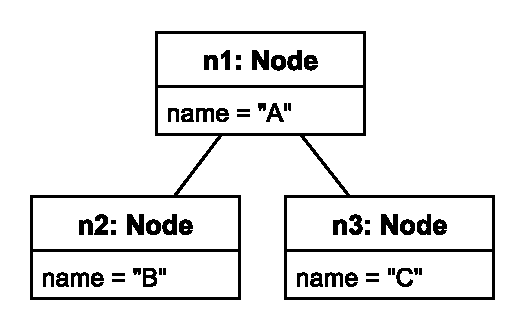
\includegraphics[width=0.6\linewidth]{initial_chart}
\caption{A tree model with 5 nodes. Node \emph{n3} and \emph{n5} are deleted from a model.}
\label{fig:initial_model}
\end{figure}

As the first, main example for this paper, we create an tree model as shown in Fig. \ref{fig:initial_model} based on the metamodel in Fig. \ref{fig:node_metamodel}. The model is constructed in two sessions. In the first session \emph{s1}, the model is constructed consisting of five nodes \emph{n1}, \emph{n2}, \emph{n3}, \emph{n4}, and \emph{n5}. Node \emph{n1} contains three direct nodes \emph{n2}, \emph{n3}, and \emph{n4}, and node \emph{n3} contains node {n5}. Later in the second session \emph{s2}, node \emph{n3} is deleted from the model, which means node \emph{n5} is also deleted since node \emph{n5} is contained by node \emph{n3} (the later-deleted nodes are coloured gray). The order of the creation of this model can be seen in its CBP representation in Lst. \ref{lst:cbpmodel}.

\noindent
\begin{minipage}[t]{0.34\linewidth}
\begin{lstlisting}[style=xmi,caption={State-based representation of the model of Figure \ref{fig:initial_model} after removal of node \emph{n5} in (simplified) XMI.},label=lst:xmimodel]
<Node id="n1" name="A">
  <children id="n2" 
    name="B"/>
  <children id="n3"
      name="C"/>
  <children id="n4"
      name="D"/>
</Node>
\end{lstlisting}
\end{minipage}
\hfill
\begin{minipage}[t]{0.635\linewidth}
\begin{lstlisting}[style=eol,caption={Change-based representation of the model of Figure \ref{fig:initial_model} after removal of node \emph{n5}.},label=lst:cbpmodel]
session s1
create n1 of Node
set n1.name to "A" //m5.name="A"
create n2 of Node
set n2.name to "B" //m5.name="B"
create n3 of Node
set n3.name to "C" //m5.name="C"
create n4 of Node
set 4.name to "D" //m5.name="D"
create n5 of Node
set n5.name to "E" //m5.name="E"
add n2 to n1.children   //n1.children={n2}
set n2.parent to n1     //n2.parent=n1
add n3 to n1.children   //n1.children={n2,n3}
set n3.parent to n1     //n3.parent=n1
add n4 to n1.children   //n1.children={n2,n3,n4}
set n4.parent to n1     //n4.children=n1
add n5 to n3.children   //n3.children={n5}
set n5.parent to n3     //n5.children=n3
session s2
remove n5 from n3.children //n3.children={}
delete n5 
remove n3 from n1.children //n3.children={n2,n4}
delete n3
\end{lstlisting}
\end{minipage}

\section{Proposed Approach}
\label{sec:proposed_approach}
To illustrate the proposed approach, List. \ref{lst:xmimodel} shows a state-based representation of the model of Fig. \ref{fig:initial_model} after the removal of node \emph{n5} in (simplified) XMI, and List. \ref{lst:cbpmodel} shows the proposed equivalent change-based representation of the same model. Instead of a snapshot of the state of the model, the representation of List. \ref{lst:cbpmodel} captures the complete sequence of change events (create, set, unset, add, remove, move, delete) that were performed on the model since its creation (We use the notification facility provided by the EMF framework to capture the change events for our prototype). Replaying these changes produces the same state as the one captured in List. \ref{lst:xmimodel}, so the proposed representation contains at least as much information as the state-based representation. 

Nevertheless, replaying all the changes to obtain the eventual state is resource consuming for large models. Therefore, an optimisation algorithm is needed and can be realised by ignoring events that are cancelled out by other subsequent events. For example, all events related to node \emph{n5} (lines 10-11, 19, 21-22) can be ignored since the node does not appear in the eventual state of the model. Thus, the loading optimisation needs a data structure that track objects' events and their positions of occurrence in a CBP representation and an algorithm to identify from the model history which events that are cancelled out.

\begin{figure}[ht]
\centering
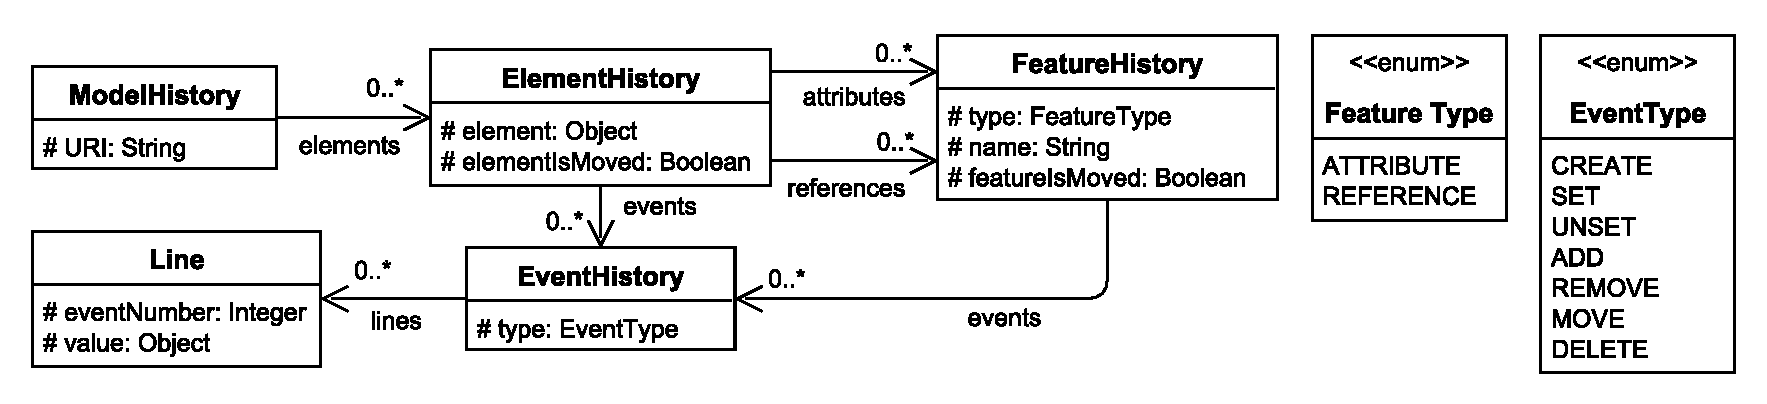
\includegraphics[width=\linewidth]{object_history}
\caption{A class diagram of recording object history.}
\label{fig:object_history}
\end{figure}

A model history (Fig. \ref{fig:object_history}) is a data structure that tracks objects, their events, and their event numbers, the events' positions, in a CBP representation). A \emph{ModelHistory} can have many \emph{ObjectHistory}, which is reflection that a model can have more than one object as its elements.\emph{ObjectHistory} has an attribute \emph{object} that identify an instance of the \emph{ObjectHistory} belongs to specific object. The attribute \emph{isMoved} is a flag used to identify the state of the object if the object is already affected by a \emph{move} operation (discussed in subsection \ref{subsec:add_remove_and_move_operations}). Each \emph{ObjectHistory} consists of one or more \emph{EventHistory} to reflect that an object can be involved in different types of events/operations. The \emph{EventHistory} records a set of \emph{Line} that contains lines where an object and its events occur in a CBP format. The \emph{Line} has attributes \emph{eventNumber} and \emph{value} that hold its event number in the CBP format and the value of involved operand respectively. 

\section{Loading Time Optimisation}
\label{sec:loading_time_optimisation}
We can apply many types of operations to a model. Set and unset operations are applied to a single-valued attribute or reference, add, remove, and move operations are applied to a multi-valued attribute or reference, and create and delete operation are applied to an object. Each of these groups operations has specific algorithm to identify cancelled-out events. 

\subsection{Set and Unset Operations}
\label{subsec:set_and_unset_operations}
During a model development, a single-valued attribute or reference of an object can be assigned many times. We identify that the last value that is assigned to the attribute is all that matters---the last assigned value is the value that is hold by the attribute in the eventual model. Previous assignments can be ignored since they do not affect the eventual state of a model. For example in List. \ref{lst:set_unset_example}, the attribute \emph{name} is assigned ``A", and then ``B", and then nullified (unset), and finally ``C". We can execute only the last assignment (line 5) to optimise the execution, ignoring the previous operations, to produce the same end model as if we executes all the operations. 

\begin{lstlisting}[style=eol,caption={Example of CBP representation of \emph{name} attribute assignments.},label=lst:set_unset_example]
create n1 of Node
set n1.name to "A"    //n1.name="A"    
set n1.name to "B"    //n1.name="B"
unset n1.name         //n1.name=null
set n1.name to "C"    //n1.name="C"
\end{lstlisting}

To make the optimisation possible, the event numbers where the attribute \emph{name} affected in Lst. \ref{lst:set_unset_example} are stored into its respective object history.  For example, lines for \emph{set} and \emph{unset} events in their event histories are \emph{setEventHistory.lines = setEventLines =} [[2, ``A"], [3, ``B"], [5, ``C"]] and \emph{unsetEventHistory.lines = unsetEventLines} = [[4, null]] respectively. Since only the last value of set or unset operations that is significant, using the two lists, we can identify that line 5 is the last line of set and unset operations that is significant for the attribute \emph{name}. Therefore, lines 2 to 4 can be put into the ignore list.  

\begin{algorithm}
\begin{small}
\SetKwInOut{Input}{input}
\SetKwInOut{Output}{output}
\SetKwProg{Struct}{struct}{}{end}
\Struct{Line}{
    Integer $eventNumber$;
    Var $value$;
}
\Input{two lists of Line $setEventLines$ and $unsetEventLines$, a list of Integer $ignoreList$}
\Output{a list of Integer $ignoreList$}
\SetKwBlock{Beginn}{beginn}{ende}
\Begin{
$setLastLine$ $\leftarrow$ getLastLine($setEventLines$)\;
$unsetLastLine$ $\leftarrow$ getLastLine($unsetEventLines$)\;
\uIf{$setLastLine > unsetLastLine$}{
    Add every event number in $setEventLines$ into $ignoreList$ except the last line\;
    Add all event numbers in $unsetEventLines$ into $ignoreList$\; 
}

\ElseIf{$setLastLine < unsetLastLine$}{
    Add all event numbers in $setEventLines$ into $ignoreList$\;
    Add all event numbers in in $unsetEventLines$ into $ignoreList$\; 
}
\Return{$ignoreList$}\;
}
\end{small}
\caption{Algorithm to identify lines that can be ignored for attribute's \emph{set} and \emph{unset} operations}
\label{alg:set_unset_optimisation}
\end{algorithm}

The algorithm to execute this argument is shown in Alg. \ref{alg:set_unset_optimisation}. It takes three inputs: two list of \emph{Line}, \emph{setEventLines} and \emph{unsetEventLines}, and a list of Integer, \emph{ignoreList}. The \emph{Line} is a structure that represents an event. It carries the \emph{eventNumber} of the event in its CBP representation as well as the \emph{value} involved. The \emph{setEventLines} and \emph{unsetEventLines} are lists that contains the \emph{Line}s where the event \emph{setAttributeEvent} and \emph{unsetAttributeEvent} appear in a CBP representation and the operand's value included in the event. The algorithm starts by retrieving the last lines of \emph{setEventLines} and \emph{unsetEventLines} using the \emph{getLastLine} function and assigning them to variables \emph{setLastLine} and \emph{unsetLastLine} (lines 5 and 6). If \emph{setLastLine} is larger than \emph{unsetLastLine} then every event number that is in the \emph{setEventLines} are put into the \emph{ignoreList} excluding the last value since the last line still has to be executed to produce the same end model (lines 7-9). If \emph{unsetLastLine} is larger than \emph{setLastLine} then \emph{unset} operation is the last operation that is executed (line 10). Therefore, there is no need to executes all \emph{set} and \emph{unset} operations---all lines can be ignored. Every event numbers in \emph{setEventLines} and \emph{unsetEventLines} are put into the \emph{ignoreList}. The \emph{ignoredList} is then returned for further processes.

The algorithm (Alg. \ref{alg:set_unset_optimisation}) can also be applied to set and unset operations of a non-containment reference for CBP described in Lst. \ref{lst:set_unset_reference}. For nodes \emph{n1}, \emph{n2}, \emph{n3}, and \emph{n4} are created at the beginning of the creation of its model (line 1-4). The \emph{n1}'s non-containment reference, \emph{parent}, is then assigned \emph{n2} and \emph{n3} accordingly (lines 5-6), before nullified or unset (line 7). Finally, the \emph{n1.parent} is set to \emph{n4}. 

\begin{lstlisting}[style=eol,caption={Example of CBP representation of \emph{name} reference assignments.},label=lst:set_unset_reference]
create n1 of Node
create n2 of Node
create n3 of Node
create n4 of Node
set n4.parent to n1    //n4.parent=n1
set n4.parent to n2    //n4.parent=n2
unset n4.parent        //n4.parent=null
set n4.parent to n3    //n4.parent=n3
\end{lstlisting}

Using the same optimisation to set and unset operations of non-containment reference \emph{parent}, we can omit lines 5 to 7 to produce the same end model. In in their event histories, the lines for set and unset operations are \emph{setEventLines} = [[5, n1], [6, n2], [8, n3]] and \emph{unsetEventLines} = [[7, null]] respectively. Since only the last value of set or unset operations that is significant, using the two lists, we can identify that line 8 is the last line of set and unset operations that is significant for the non-containment reference \emph{parent}. Therefore, lines 5 to 7 can be put into the ignore list.

\subsection{Add, Remove, and Move Operations}
\label{subsec:add_remove_and_move_operations}
An attribute can also contains many values; we can add and remove values from it. For example (List. \ref{lst:add_remove_move_attribute}), \emph{node} object has \emph{values} attribute that can contains many integer values. We add values 11, 12, and 13 subsequently (line 2-4) to the attribute and remove the value 12 at line 5. We show in the commented parts the states of \emph{node.values}.  

\begin{lstlisting}[style=eol,caption={Example of CBP representation of attribute \emph{values}'s add and remove operations.},label=lst:add_remove_move_attribute]
create node of Node
add 11 to node.values      //node.values=[11] 
add 12 to node.values      //node.values=[11,12] 
add 13 to node.values      //node.values=[11,12,13] 
remove 12 from node.values //node.values=[11,13] 
\end{lstlisting}

The execution of these operations can be optimised by ignoring the add and remove operations of the value 12 (lines 3 and 5) since we can produce the same end model only by adding 11 and 13 (line 2, 4). When events in List. \ref{lst:add_remove_move_attribute} are executed, they populate line lists for add and remove event histories of attribute \emph{values}, \emph{addEventLines} = [[2,11], [3,12], [4,13]] and \emph{removeEventLines} = [[5,12]]. Using the two lists, we can identify the event number of lines that can be put into the ignore list, producing \emph{ignoreList} = [3, 5]. The algorithm to execute this argument is shown in Alg. \ref{alg:add_remove_move_optimisation}.

\begin{algorithm}
\begin{small}
\SetKwInOut{Input}{input}
\SetKwInOut{Output}{output}
\SetKwProg{Struct}{struct}{}{end}
\Struct{Line}{
    Integer $eventNumber$;
    Anytype $value$;
}
\Input{two lists of Line $addEventLines$, $removeEventLines$, and $moveEventLines$, a list of Integer $ignoreList$, a variable of Anytype $operandValue$, a variable of Boolean $attributeIsMoved$, an object of Feature $feature$}
\Output{a list of Integer $ignoreList$}
\SetKwBlock{Beginn}{beginn}{ende}
\Begin{
\If{$attributeIsMoved$ = false}{
    $filteredAddLines$ $\leftarrow$ filterLinesByValue($addEventLines$, $operandValue$)\;
$filteredRemoveLines$ $\leftarrow$ filterLinesByValue($removeEventLines$, $operandValue$)\;
$addLastLine$ $\leftarrow$ getLastLine($filteredAddLines$)\;
$removeLastLine$ $\leftarrow$ getLastLine($filteredRemoveLines$)\;
\uIf{$addLastLine > removeLastLine$}{
    Add every event number in $filteredAddLines$ into $ignoreList$ except the last value\;
    Add all event numbers in $filteredRemoveLines$ into $ignoreList$\; 
}
\ElseIf{$addLastLine < removeLastLine$}{
    Add all event numbers in $filteredAddLines$ into $ignoreList$\;
    Add all event numbers in $filteredRemoveLines$ into $ignoreList$\; 
}
}
\If{feature is empty or feature only has a value}{
    \uIf{feature is empty}{
        Add all event numbers in $addEventLines$ into $ignoreList$\;
    }\ElseIf{feature only has a value}{
        Add every event number in $addEventLines$ into $ignoreList$ except the last value\;
    }
        Add all event numbers in $removeEventLines$ into $ignoreList$\; 
        Add all event numbers in $moveEventLines$ into $ignoreList$\; 
        $attributeIsMoved$ $\leftarrow$ false\;
}
\Return{$ignoreList$}\;
}
\end{small}
\caption{Algorithm to identify lines that can be ignored for \emph{add}, \emph{remove}, and \emph{move} operations.}
\label{alg:add_remove_move_optimisation}
\end{algorithm}

The algorithms takes seven inputs: three line lists that contain the lines of add (\emph{addEventLines}), remove (\emph{removeEventLines}), and move (\emph{moveEventLines}) events, an ignore list \emph{ignoreList}, the variable \emph{operandValue} to hold the value used in an event, a flag variable \emph{attributeIsMoved}, and an object of Feature \emph{feature} which can be an attribute or reference. The algorithm starts by checking the value of \emph{attributeIsMoved} to the member of the attribute's values if they are already moved or not (line ). We explain more the use of \emph{attributeIsMoved} later in this section. If the values are not moved yet, the algorithm continues with filtering all the line lists by the operandValue and stored them into filtered line lists: \emph{filteredAddLines} and \emph{filteredRemoveLines}. The algorithm the retrieves the last lines of the filtered line lists using the \emph{getLastLine} function and assigns them to \emph{addLastLine} and \emph{removeLastLine}. If the \emph{addLastLine} is larger than {removeLastLine} then all event numbers of \emph{filteredAddLines} and \emph{filteredRemoveLines}, except for the last line of \emph{filteredAddLines}, are added into the \emph{ignoreList}. Otherwise, all event numbers in both filtered line lists are added into the\emph{ignoreList}.

The algorithm then proceeds by checking the feature. If the feature is empty then all event numbers in the \emph{addEventLines} are added into the \emph{ignoreList}. If the feature only has one value, all the event numbers also added into the \emph{ignoreList} except the last line. The algorithm then proceeds by adding all event numbers in \emph{removeEventLines} and \emph{moveEventLines} into the \emph{ignoreList}. After that, \emph{attributeIsMoved} is set to false. Finally, the \emph{ignoreList} is returned for further operations.     

\begin{lstlisting}[style=eol,caption={Example of CBP representation of attribute \emph{values}'s add and remove operations.},label=lst:add_remove_move_reference]
create n1 of Node
create n2 of Node
create n3 of Node
create n4 of Node
add n2 to node.children      //n1.children=[n2] 
add n3 to node.children      //n1.children=[n2,n3] 
add n4 to node.children      //n1.children=[n2,n3,n4] 
remove n3 from node.children //n1.children=[n1,n4] 
\end{lstlisting}

The algorithm (Alg. \ref{alg:add_remove_move_optimisation}) can also be applied to add, remove, and move operations of a containment reference for CBP described in Lst. \ref{lst:add_remove_move_reference}. For nodes \emph{n1}, \emph{n2}, \emph{n3}, and \emph{n4} are created at the beginning of the creation of its model (line 1-4). The \emph{n1}'s multivalue containment reference, \emph{children}, is then added \emph{n2},\emph{n3}, and \emph{n4} accordingly (lines 5-7), before the removal of node \emph{n3} (line 8). 

Using the same optimisation to \emph{add}, \emph{remove}, and \emph{move} operations of containment reference \emph{children}, we can omit lines 6 to 8 to produce the same end model. In in their event histories, the lines for set and unset operations are \emph{addEventLines} = [[5, n2], [6, n3], [7, n4]] and \emph{removeEventLines} = [[8, n3]] respectively. Since the \emph{remove} operation at line 8 makes itself and the \emph{add} operation at line 6 insignificant, lines 6 and 8 can be put into the ignore list.

\begin{lstlisting}[style=eol,caption={Example of CBP representation of attribute \emph{values}'s move operations.},label=lst:move_attribute_example]
create node of Node
add 11 to node.values            //node.values=[11] 
add 12 to node.values            //node.values=[11,12] 
add 13 to node.values            //node.values=[11,12,13] 
move from 0 to 1 in node.values  //node.values=[12,11,13]  
remove 12 from node.values       //node.values=[11,13] 
\end{lstlisting}

\begin{lstlisting}[style=eol,caption={Example of optimised CBP representation of attribute \emph{values}'s move operations.},label=lst:move_attribute_example_error]
create node of Node              //(1)  
add 11 to node.values            //(2) node.values=[11] 
add 13 to node.values            //(4) node.values=[11,13] 
move from 0 to 1 in node.values  //(5) node.values=[13,11]   
\end{lstlisting}

The `\emph{if attributeIsMoved = false}' condition at line 5 in Alg. \ref{alg:add_remove_move_optimisation} indicates that removing previous add and remove events can only be applied if no move operation has been executed previously to the attribute. This condition is required, since after optimisation, some operations are already removed and therefore makes some values may not exist, which changing the indexes of other values. Consequently, replaying all the events may not produce the same end model with the non-optimised CBP representation. 

To illustrate this case, we compare the eventual model loaded from a CBP representation (List. \ref{lst:move_attribute_example}) to another model loaded from and optimised CBP representation (List. \ref{lst:move_attribute_example_error})---the same representation but has been optimised. The optimisation removes line 3 and 6 in List. List. \ref{lst:move_attribute_example} and when loaded back again the end models are not same. The non-optimised CBP representation produces \emph{node.values} = [11,13] while the optimised one produces \emph{node.values} = [13,11]. When \emph{remove 12} is executed (List. \ref{lst:move_attribute_example} line 6), the optimisation ignores the \emph{add 12} operation (List. \ref{lst:move_attribute_example} line 3) and thus makes the index of 13 is 1 in the optimised CBP, while the index of 13 is 2 in the non-optimised CBP, and produces different end model when \emph{move from 0 to 1} (List. \ref{lst:move_attribute_example_error}, line 4) is executed. 

The \emph{attributeIsMoved}'s state is set to true when a move operation is applied within it's attribute and the number of of it's attributes' values is more than 1. The \emph{attributeIsMoved}'s state is set to false again when the attribute is empty or only has a value (\ref{alg:add_remove_move_optimisation}, line 18-26) since any move operation does not affect the indexes of the attributes' values.



%\begin{lstlisting}[style=eol,caption={Example of CBP representation of attribute \emph{values}'s move operations.},label=lst:move_attribute_object_example]
%create node of Node
%create n1 of Node
%create n2 of Node
%create n3 of Node
%add n1 to node.children            //node.children=[n1] 
%add n2 to node.children            //node.children=[n1,n2] 
%add n3 to node.children            //node.children=[n1,n2,n3] 
%move from 0 to 1 in node.children  //node.children=[n2,n1,n3]  
%remove n2 from node.children       //node.children=[n1,n3] 
%\end{lstlisting}
%
%\begin{lstlisting}[style=eol,caption={Example of optimised CBP representation of attribute \emph{values}'s move operations.},label=lst:move_attribute_example_object_error]
%create node of Node                //(1)  
%create n1 of Node                  //(2)  
%create n3 of Node                  //(4)  
%add n1 to node.children            //(5) node.children=[n1] 
%add n3 to node.children            //(7) node.children=[n1,n3] 
%move from 0 to 1 in node.children  //(8) node.children=[n3,n1]   
%\end{lstlisting}

\subsection{Create and Delete Operations}
\label{subsec:create_and_delete_operations}
The examples of object's create event has been demonstrated in several Listings in this paper where \emph{create} is the keyword that denotes the event in a CBP representation. The create operation is only executed  once per object. It cannot be created more than once. Meanwhile, the example of object's delete event is exhibited in Lst. \ref{lst:cbpmodel}. When an object is deleted, it means that the object is completely removed from the model---no longer exists. Therefore, all events (create, delete, set, unset, add) related to the object can be ignored---there is no need to create the object and all its attributes' events can be ignored as well. 

If  Lst. \ref{lst:cbpmodel} is optimised by removing node n3 (n5 is removed first since n5 is contained in n3), then the otimisation produces the CBP representation as in Lst. \ref{lst:cbpmodel_optimised}. The optimisation ignores 10 lines (lines 6, 7, 10, 11, 13, 15, 17, 18, 19, and 20) since those lines are related to nodes \emph{n3} and \emph{n5} and ignoring the lines still produces the same end model to the one produced by the non-optimised CBP representation (Lst. \ref{lst:cbpmodel}). 

\begin{lstlisting}[style=eol,caption={Change-based representation of the model of Figure \ref{fig:initial_model} after removal of node \emph{n5}.},label=lst:cbpmodel_optimised]
session s1                   //(1)
create n1 of Node            //(2)
set name of n1 with "A"      //(3)  n1.name="A"
create n2 of Node            //(4)
set name of n2 with "B"      //(5)  n2.name="B"
create n4 of Node            //(8)
set name of n4 with "D"      //(9)  n4.name="D"
add n2 to n1.children        //(12) n1.children={n2}
add n4 to n1.children        //(14) n1.children={n2,n4}
session s2                   //(16)
\end{lstlisting}

We use Alg. \ref{alg:create_delete_optimisation} to determine lines that are ignored after a \emph{delete} operation. The algorithm takes two inputs, \emph{deletedObject}, an variable of object that is deleted, and \emph{ignoreList}, a list of Integer that contains ignored event numbers. After some processes, the algorithm will return the \emph{ignoreList} as its output. The algorithm starts by checking whether the \emph{deletedObject} is already moved or not (line 2), if it is not then it is safe to remove all lines that refer to the object (line 3). Otherwise, no action is executed. The algorithm then retrieves all event histories \emph{eventHistoryList} that refer to the object (line 4)and iterates through each event history (line 5-8). For every event history \emph{eventHistory} (line 5), the algorithm retrieves its lines \emph{lineList} (line 6) and put all their event numbers into the \emph{ignoreList} (line 7). After that, the algorithm continues to iterate through all its attributes and put all lines of their events into the \emph{ignoreList} as well (lines 12-15). As a result, the next time the CBP representation (Lst. \ref{lst:cbpmodel}) is loaded, the loading process can refer to the \emph{ignoreList} whether certain lines in the CBP representation are ignored or not.       

\begin{algorithm}
\begin{small}
\SetKwInOut{Input}{input}
\SetKwInOut{Output}{output}
\Input{a variable ofObject $deletedObject$, a list of Integer $ignoreList$}
\Output{a list of Integer $ignoreList$}
\Begin{
$objectIsMoved$ $\leftarrow$ isObjectMoved($deletedObject$)\;
\If{$objectIsMoved$ = false}{
    $eventHistoryList$ $\leftarrow$ getAllEventHistories($deletedObject$)\; 
    \ForEach{$eventHistory$ in $EventHistoryList$}{
        $lineList$ $\leftarrow$ getLines($eventHistory$)\;
        Add all event numbers in $lineList$ into $ignoreList$\; 
    }
    $attributeList$ $\leftarrow$ getAllAttributes($deletedObject$)\;
    \ForEach{$attribute$ in $attributeList$}{
        $eventHistoryList$ $\leftarrow$ getAllEventHistories($attribute$)\;
        \ForEach{$eventHistory$ in $EventHistoryList$}{
            $lineList$ $\leftarrow$ getLines($eventHistory$)\;
            Add all event numbers in $lineList$ into $ignoreList$\; 
        }       
    }   
}
\Return{$ignoreList$}\;
}
\end{small}
\caption{Algorithm to identify lines that are ignored after \emph{delete} operations}
\label{alg:create_delete_optimisation}
\end{algorithm}

For example, based on Lst. \ref{lst:cbpmodel} and using Alg. \ref{alg:create_delete_optimisation}, deleting node \emph{n5} fills up the \emph{ignoreList} with all the event numbers contained in its object history. Thus, the deletion produces \emph{ignoreList} = [10, 11, 18, 19, 21, 22]. Using the same approach, the deletion of node \emph{n3} adds more event numbers and produces \emph{ignoreList} = [6, 7, 10, 11, 14, 15, 18, 19, 21, 22, 23, 24].

\section{Performance Evaluation}
\label{sec:performance_evaluation}
We have implemented a prototype\footnote{The prototype is available under \url{https://github.com/epsilonlabs/emf-cbp}} of the change-based model persistence using the Eclipse Modelling Framework. We evaluate the prototype's performance on saving time, loading time, and memory consumption. For the saving time, we contrast the saving time between appending in CBP and saving in XMI. For the loading time, we perform comparison on loading time between optimised CBP, non-optimised CBP, and XMI. For memory consumption, we compare the performance of optimised CBP and XMI on memory consumption.

\subsection{Saving Time Test}
\label{subsec:saving_time_test}
We evaluate the performance of our prototype on saving time to gain insight on the efficiency that can be gained from the CBP representation against XMI as the comparison baseline. The  comparison is depicted in Fig. \ref{fig:append_speed}.

\begin{figure}	
	\begin{subfigure}[t]{0.5\linewidth}
		\includegraphics[width=\linewidth]{append_speed_tree}
		\caption{Tree domain}\label{fig:append_speed_tree}		
	\end{subfigure}
	\hfill
	\begin{subfigure}[t]{0.5\linewidth}
		\includegraphics[width=\linewidth]{append_speed_conf}
		\caption{Conference domain}\label{fig:append_speed_conference}
	\end{subfigure}
	\caption{A comparison on time used to persist models between CBP and XMI. The y-axis is log\textsc{2} scaled.}
	\label{fig:append_speed}
\end{figure}

In performing our comparison, we seek the relationship between number of objects in a model and the time required persist the model. We create courses of random operations in Epsilon Object Language \cite{kolovos2006epsilon} for each tree and conference domains and executed them to simulate the development of models. For CBP, we measure the time consumed to append events generated for every operation. For XMI, we measure the time used to persist the eventual state for each model generated. 

In Fig. \ref{fig:append_speed}, for both tree and conference domains, the time consumed to persist events in CBP is nearly constant, whereas for XMI, the time consumed to persist a model increases linearly along the growth of objects. Based on our measurement, the time consumed to append events into a CBP representation is 1.16 miliseconds on overage and the time to save model in XMI is increased 2.25 microseconds for each additional object. This finding suggest persisting changes of a model is much faster rather than persisting its complete eventual state after the model is modified.    

\subsection{Loading Time Test}
\label{subsec:loading_time_test}
We compare optimised CBP, non-optimised CBP, and XMI on their loading time to evaluate the performance of the optimisation algorithm. The  comparison is depicted in Fig. \ref{fig:loading_speed}. We seek the relationship between number of objects of a model and time required to load the model. We create courses of random operations and execute them to simulate the model construction.   

\begin{figure}	
	\begin{subfigure}[t]{0.5\linewidth}
		\includegraphics[width=\linewidth]{loading_speed_tree}
		\caption{Tree domain}\label{fig:append_speed_tree}		
	\end{subfigure}
	\hfill
	\begin{subfigure}[t]{0.5\linewidth}
		\includegraphics[width=\linewidth]{loading_speed_conf}
		\caption{Conference domain}\label{fig:append_speed_conference}
	\end{subfigure}
	\caption{A comparison on load time between XMI, optimised CBP, and non-optimised CBP. The y-axis is log\textsc{10} scaled.}
	\label{fig:loading_speed}
\end{figure}

Fig. \ref{fig:loading_speed} shows a pattern that the optimised CBP consumes less time than the non-optimised CBP on loading models. However, different domains of models show different efficiency. In the case of conference domain, the optimised CBP's loading time is less efficient than the one in tree domain, even though it is still faster than the non-optimised CBP. Thus, the efficiency depends on the characteristics of the domain's model. We argue that domains that typically perform lots of modifications and deletions will benefit more, such as the tree domain that has multiple levels of containment, which means deleting a node also deleting its direct and indirect nodes, whereas in conference domain, it typically contains hundreds of participants but less likely to have multilevel containment creating a shallow, flat tree-like characteristic. 

In the case of tree model, the optimised CBP is becoming more efficient than the non-optimised CBP when the number of loaded objects is increasing. The optimise CBP's loading time is linearly increasing while the non-optimised one tends to grow exponentially. However, still, it cannot outperform the XMI's loading time, since more time is used to de-serialise the CBP format. Optimising the serialised format will reduce the loading time of the optimised CBP.  

\subsection{Memory Consumption}
\label{subsec:memory_consumption}

\begin{figure}	
	\begin{subfigure}[t]{0.5\linewidth}
		\includegraphics[width=\linewidth]{memory_use_tree}
		\caption{Tree domain}\label{fig:append_speed_tree}		
	\end{subfigure}
	\hfill
	\begin{subfigure}[t]{0.5\linewidth}
		\includegraphics[width=\linewidth]{memory_use_conf}
		\caption{Conference domain}\label{fig:append_speed_conference}
	\end{subfigure}
	\caption{A comparison on memory consumption between CBP and XMI.}
	\label{fig:memory_use}
\end{figure}

Another evaluation that we perform is we optimised CBP and XMI on their memory consumption after loading models. We use the \emph{memory-measurer}\footnote{\url{https://github.com/DimitrisAndreou/memory-measurer}} tool to measure the memory footprints. We also use other tools, such as Jamm\footnote{\url{https://github.com/jbellis/jamm}} and Classmexer\footnote{\url{http://www.javamex.com/classmexer/}} to verify the measurement. It turns out that the results are not significantly different and still follow the same trend). We use a deep measure, every object referenced in the measured object is also calculated, to calculate the total consume. 

The results are shown in Figure \ref{fig:memory_use}. In both tree and conference domains, XMI significantly outperforms CBP in terms of memory consumption after loading models. The large memory consumption of CBP is caused by the model history that consumes space in memory to holds objects, their events, and their event numbers. This condition leads us to another future work that is to identify and remove objects, events, and events numbers from the model history once they are not any longer required. For example, once a object is deleted from a model, all its records in the model history are removed to release space in memory. 

\section{Related Work}
\label{sec:related_work}
\lipsum[3]
\lipsum[4]

\section{Limitations}
\label{sec:limitations}
So far, we only address attribute or reference that can only contains unique members---no duplicate values or objects. Duplicate members means that removal of a value /object does not mean the removal of other same values/objects since values/objects with different positions contained in the feature are perceived different. Therefore, positions of values/objects have to be considered by the optimisation algorithm. Furthermore, we also have not addressed features that has default values. Default value of a feature might not trigger any event. Failure to address this might produce different end models. 

Models in the real world are most likely different from the random models generated in the evaluation. Their optimised CBP's loading time can perform better or worse than the ones presented in this paper. In another condition, the optimised CBP is not always outperform the non-optimised CBP in every condition. There is a condition where optimised CBP is not faster than the non-optimised CBP that is when only \emph{create} operation is performed, without performing other types of operation, since there is no event that can be ignored. One feasible way to better reflect real-world models is to ask modellers to create complex models using different modelling languages, persist their histories, and analyse the results to gain insight whether the optimisation really works for real-world models. 

\section{Conclusions}
\label{sec:conclusions}
In this paper, we have proposed a change-based, as an alternative to stated-based, persistence as an approach to persist a model. We also have proposed the algorithm to optimise its loading time as well evaluated the change-based persistence on saving time, loading time, and memory time against the XMI and non-optimised CBP as the baselines. Our results show considerable savings in terms of persisting and identifying changes made to models at an increased---but linear---model loading cost. For future work, we  plan to extend the CBP to enable change detection, model merging, conflict resolution of models in the context of collaborative modelling.

\subsubsection*{Acknowledgments.} This work was partly supported through a scholarship managed by \emph{Lembaga Pengelola Dana Pendidikan Indonesia} (Indonesia Endowment Fund for Education).

\bibliography{references} 
\bibliographystyle{splncs}

\end{document}
